\documentclass[aspectratio=169,11pt]{beamer}
\usetheme{Madrid}
\usepackage[utf8]{inputenc}
\usepackage[T1]{fontenc}
\usepackage{booktabs,graphicx}
\graphicspath{{../reports/figures/}{./}}

% ---- colours from the website (src/web/demo.css) ----
\definecolor{ink}{HTML}{0B0B0C}
\definecolor{lime}{HTML}{D6ED43}
\definecolor{limedark}{HTML}{778200}
\definecolor{canvas}{HTML}{F7F7F8}
\definecolor{graphite}{HTML}{2A2A2D}
\definecolor{muted}{HTML}{71717A}
\setbeamercolor{palette primary}{bg=ink,fg=lime}
\setbeamercolor{palette secondary}{bg=graphite,fg=white}
\setbeamercolor{palette tertiary}{bg=lime,fg=ink}
\setbeamercolor{palette quaternary}{bg=ink,fg=white}
\setbeamercolor{structure}{fg=ink}
\setbeamercolor{frametitle}{bg=ink,fg=white}
\setbeamercolor{title}{bg=ink,fg=white}
\setbeamercolor{subtitle}{fg=lime}
\setbeamercolor{background canvas}{bg=canvas}
\setbeamercolor{normal text}{fg=ink}
\setbeamercolor{itemize item}{fg=limedark}
\setbeamercolor{itemize subitem}{fg=limedark}
\setbeamercolor{block title}{bg=ink,fg=lime}
\setbeamercolor{block body}{bg=white,fg=ink}
\setbeamercolor{section in head/foot}{bg=lime,fg=ink}
\setbeamercolor{author in head/foot}{bg=ink,fg=lime}
\setbeamercolor{title in head/foot}{bg=graphite,fg=white}
\setbeamercolor{date in head/foot}{bg=lime,fg=ink}
\setbeamertemplate{navigation symbols}{}
\setbeamerfont{frametitle}{series=\bfseries}
\setbeamerfont{footline}{size=\scriptsize}
\logo{
\includegraphics[height=0.75cm]{logo.png}\hspace{2pt}\vspace{-3pt}}

\title[PegaSold]{PegaSold: Baku Home Price Prediction}
\subtitle{Decision tree, Pegasos SVM and bagging, built from scratch in NumPy}
\author[Team PegaSold]{Emiliya Abdulhalimova \and Aygun Asvarova \and Murad Bagirzade \and Kanan Karimli}
\institute[MLE-AI-201]{MLE-AI-201 Machine Learning · AI Academy}
\date[Oct 2026]{October 2026}

\begin{document}

\begin{frame}
  \titlepage
  \centering
\includegraphics[height=1.3cm]{logo.png}
\end{frame}

\section{Problem and data}
\begin{frame}{The problem}
\begin{itemize}\setlength\itemsep{0.8em}
  \item bina.az listings: 100{,}775 raw rows, 51 messy Azerbaijani columns
  \item \textbf{Task A:} predict the asking price (we model $\ln$ price)
  \item \textbf{Task B:} premium or standard, split at the training median, 209{,}000 AZN
  \item Tree, SVM and ensemble are \textbf{our own NumPy code}; scikit-learn is only the baseline
\end{itemize}
\end{frame}

\begin{frame}{Cleaning: 100{,}775 rows to 57{,}003}
\begin{columns}[T]
\column{.48\textwidth}\small
\begin{tabular}{lr}\toprule Step & Rows\\\midrule
Raw scrape & 100{,}775\\
Deduplicate & 63{,}241\\
Baku, 3 residential types & 57{,}069\\
Price and area windows & 57{,}003\\\bottomrule\end{tabular}
\begin{itemize}
  \item Latest scrape per advert; 544 reposts removed
  \item m$^2$ for flats, \emph{sot} for land
  \item Split 70/15/15, seed 42
  \item 61 automated checks: CLEAN
\end{itemize}
\column{.52\textwidth}\centering
\includegraphics[width=\linewidth]{data_and_prices.png}
\end{columns}
\end{frame}

\begin{frame}{82 features, no leakage}
\begin{columns}[T]
\column{.5\textwidth}
\begin{itemize}\setlength\itemsep{0.5em}
  \item 11 continuous: log area, rooms, floors, lat/lng, distance to centre, area per room \dots
  \item 9 binary flags, 3 property types, 59 locations
  \item Fills, scaling and tier threshold measured on the \textbf{training split only}
  \item Removed \texttt{unit\_price}, \texttt{total\_price}, \texttt{description}
\end{itemize}
\column{.5\textwidth}\centering
\includegraphics[width=\linewidth]{price_vs_area.png}
\end{columns}
\end{frame}

\section{Models}
\begin{frame}{Four models, all from scratch}
\begin{description}\setlength\itemsep{0.6em}
  \item[Decision tree] sorted-prefix split search, Gini / entropy / MSE, depth and leaf limits, class frequencies for \texttt{predict\_proba}, feature importances
  \item[Pegasos SVM] hinge loss + $L_2$, step $1/(\lambda t)$, projection onto $\lVert w\rVert\le 1/\sqrt\lambda$, capped intercept step
  \item[RFF SVM] 128 random Fourier features approximating an RBF kernel, same Pegasos solver
  \item[Bagging] 30 trees $\times$ 6{,}000 bootstrap rows, depth 16, soft voting, out-of-bag score
\end{description}
\end{frame}

\begin{frame}{What a tree learns}
\centering
\includegraphics[height=.78\textheight]{decision_tree.png}
\end{frame}

\section{Results}
\begin{frame}{Task A: price}
\centering\small
\begin{tabular}{lccc}\toprule Model & RMSE valid & RMSE test & $R^2$ test\\\midrule
Dummy & 0.632 & --- & ---\\
Ridge & 0.241 & --- & ---\\
scikit-learn tree & 0.239 & 0.244 & ---\\
Ours: tree (depth 10) & 0.238 & 0.245 & 0.856\\
\textbf{Ours: bagging} & \textbf{0.205} & \textbf{0.218} & \textbf{0.886}\\\bottomrule\end{tabular}

\vspace{1em}
Typical error 17.8\% (tree) $\to$ \textbf{14.9\%} (bagging). Bagging cuts test MSE by 20.9\%.
\end{frame}

\begin{frame}{Task B: price tier}
\centering\small
\begin{tabular}{lccc}\toprule Model & Acc test & F1 test & AUC test\\\midrule
scikit-learn tree & 0.916 & 0.917 & 0.969\\
Ours: tree (depth 8) & 0.916 & 0.917 & 0.970\\
LinearSVC & 0.908 & 0.909 & 0.970\\
Ours: Pegasos SVM & 0.908 & 0.909 & 0.970\\
RBF SVC (8k rows) & 0.875 & 0.875 & 0.955\\
Ours: RFF SVM (8k rows) & 0.842 & 0.844 & 0.921\\
\textbf{Ours: bagging} & \textbf{0.934} & --- & \textbf{0.983}\\\bottomrule\end{tabular}
\end{frame}

\begin{frame}{Ours vs scikit-learn}
\begin{columns}[T]
\column{.5\textwidth}\centering
\includegraphics[width=\linewidth]{fig4_model_comparison.png}
\column{.5\textwidth}\centering
\includegraphics[width=\linewidth]{roc_curves.png}
\end{columns}
\small 5-fold CV: tree $0.909\pm0.001$ (sklearn $0.909$), Pegasos $0.904\pm0.002$ (LinearSVC $0.904$).
\end{frame}

\begin{frame}{Two choices we measured}
\begin{itemize}\setlength\itemsep{0.8em}
  \item \textbf{Ensemble depth.} Members at depth 8: accuracy 0.914, AUC 0.976. At depth 16: \textbf{0.929, 0.981} (+1.4 points). Averaging controls variance, so members should fit hard.
  \item \textbf{SVM regularisation.} $\lambda$ 0.01 $\to$ 0.001: accuracy 0.890 $\to$ \textbf{0.903}, AUC 0.957 $\to$ 0.967.
  \item \textbf{Nonlinear SVM.} RFF did not beat the linear SVM (0.842 vs 0.908): the extra flexibility did not pay off here.
\end{itemize}
\end{frame}

\begin{frame}{Where the model fails}
\begin{columns}[T]
\column{.55\textwidth}\centering
\includegraphics[width=\linewidth]{fig5_error_analysis.png}
\column{.45\textwidth}
\begin{itemize}\small
  \item Median error 10\% for 100k--350k AZN
  \item 33\% above 1M AZN (117 listings)
  \item Top drivers: log area (0.63), distance to centre (0.24)
  \item Luxury homes are rare and priced by features we do not see
\end{itemize}
\end{columns}
\end{frame}

\begin{frame}{Live demo}
\centering
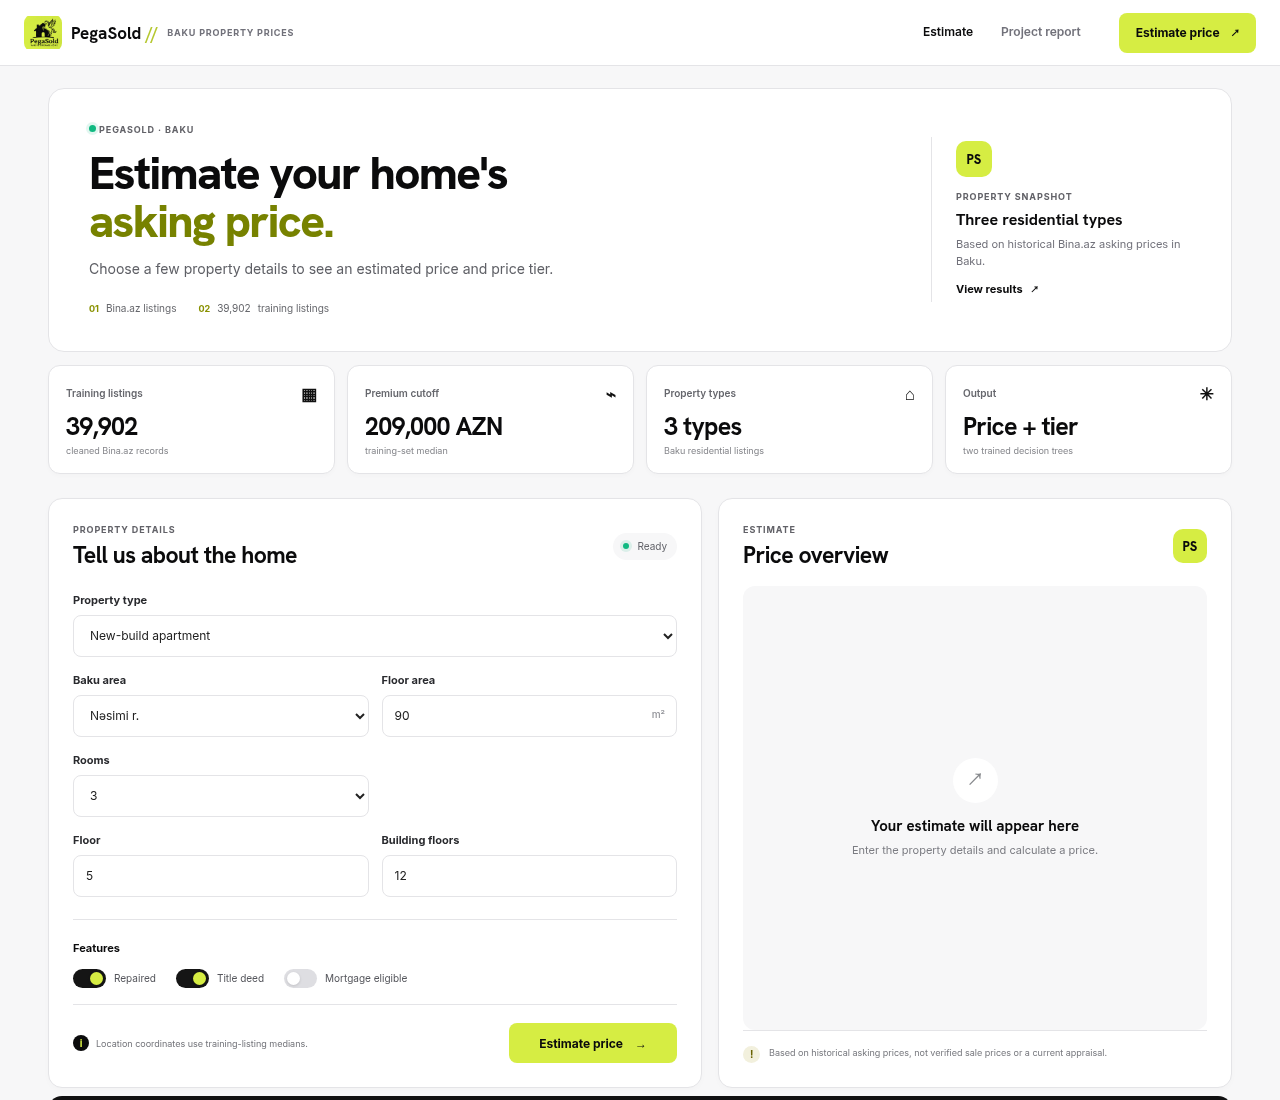
\includegraphics[height=.74\textheight]{web_demo.png}

\small \texttt{python -m src.web.web\_demo} $\to$ price + tier from our trained models
\end{frame}

\section{Wrap-up}
\begin{frame}{Limits and next steps}
\begin{itemize}\setlength\itemsep{0.6em}
  \item Depth and $\lambda$ tuned on 6{,}000 rows, used on 39{,}902
  \item Ensemble depth set by one measurement, not its own sweep
  \item Asking prices from one 2024 scrape, not sale prices
  \item Next: sweep ensemble size and depth; a separate model for luxury listings
\end{itemize}
\end{frame}

\begin{frame}{Team}
\centering
\begin{tabular}{ll}\toprule
Emiliya Abdulhalimova & data cleaning, EDA, error analysis\\
Aygun Asvarova & features, scaling, model selection\\
Kenan Karimli & decision tree, bagging\\
Murad Bagirzade & SVM, metrics, validation, pipeline\\\bottomrule
\end{tabular}

\vspace{1.2em}
\texttt{github.com/b-murad/PegaSold} \quad tag \texttt{v1.0-final}
\end{frame}
\end{document}
